\documentclass{article}
\usepackage{graphicx} % Required for inserting images

\usepackage[a4paper, left=1.5cm, right=1.5cm, top=1cm, bottom=2cm]{geometry}

\usepackage{float}

\newcounter{commentCount}
\newcounter{filePrg}
\newcounter{inputPrg}

\usepackage[dvipsnames]{xcolor}
\usepackage{minted}

\usepackage[many]{tcolorbox}
\tcbuselibrary{listings}
\tcbuselibrary{minted}

\usepackage{ifthen}
\usepackage{fontawesome}

\usepackage{tabularx}
\newcolumntype{\CeX}{>{\centering\let\newline\\\arraybackslash}X}%
\newcommand{\TwoSymbolsAndText}[3]{%
  \begin{tabularx}{\textwidth}{c\CeX c}%
    #1 & #2 & #3
  \end{tabularx}%
}

\newtcblisting[use counter=inputPrg, number format=\arabic]{codeInput}[3]{
  listing engine=minted,
  minted language=#1,
  minted options={autogobble,breaklines, fontsize=\footnotesize},
  listing only,
  size=title,
  arc=1.5mm,
  breakable,
  enhanced jigsaw,
  colframe=myblue,
  coltitle=White,
  boxrule=0.5mm,
  colback=white,
  coltext=Black,
  title=\TwoSymbolsAndText{\faCode}{%
  \textbf{Mongo Query}\ifthenelse{\equal{#2}{}}{}{\textbf{: }#2}%
  }{\faCode},
  label=inputPrg:#3
}


\usepackage{boldline}
\usepackage{tikz,tcolorbox}
\usepackage{amsmath}
\usepackage[table,xcdraw]{xcolor}
\usepackage{listings}
\usepackage{array,multirow} % For customizing tables
\usepackage{booktabs} % For better horizontal lines
\usepackage{makecell}
\setlength{\parindent}{0pt}
\usepackage{siunitx}
\usepackage{tkz-tab}
\usepackage{amssymb}
\usepackage{amsmath}
\usepackage{enumitem}

\usepackage{caption}
\usepackage{float}


\newcommand{\exer}[1]{
  \section*{Exercice #1}
  \vspace{-0.5cm}
  \noindent\rule{\textwidth}{0.5pt}%
}

\newcommand{\tit}[1]{
\begin{center}
    \Large{\textbf{{#1}}}
\end{center}
}

\definecolor{commentgray}{HTML}{676160}
\definecolor{messagegreen}{HTML}{17B867}
\definecolor{myblue}{HTML}{10C2C4}

\tcbuselibrary{skins, breakable, theorems}


\newtcolorbox{prettyBox}[2]{
  enhanced,
  colback=white!90!#2,   % Background color based on the second parameter (color)
  colframe=#2!60!black,  % Frame color based on the second parameter (color)
  coltitle=white,        % Title color (white)
  fonttitle=\bfseries\Large,
  title=#1,              % Title from the first parameter
  boxrule=1mm,
  arc=0.5mm,
  drop shadow=#2!35!gray, % Drop shadow color based on the second parameter (color)
}

\usepackage{hyperref}
\hypersetup{
    colorlinks=true,
    linkcolor=blue,
    filecolor=magenta,      
    urlcolor=cyan,
    pdftitle={Overleaf Example},
    pdfpagemode=FullScreen,
    }



\lstdefinestyle{cmd}{
 basicstyle=\ttfamily,
 backgroundcolor=\color{lightgray!20},
 frame=single
}
\usepackage{subcaption}
\usepackage{minted}

\begin{document}

\tit{LAB 1}

\section{Set Up Data Base}

\subsection{Connection}
\begin{prettyBox}{Connection}{myblue}
 By default MongoDB creates a connection to the localHost at the port 27017 , if we downloaded the
 server MongoDB we should be able to connect just by clicking the connect button.
\end{prettyBox}


\vspace{0.25cm}

\begin{figure}[H]
  \begin{subfigure}[H]{.4\textwidth}
    \centering
    
\includegraphics[width=\linewidth]{connect.png}
    \caption*{Click Connect}
  \end{subfigure}
  \hfill
  \begin{subfigure}[H]{.4\textwidth}
    \centering
    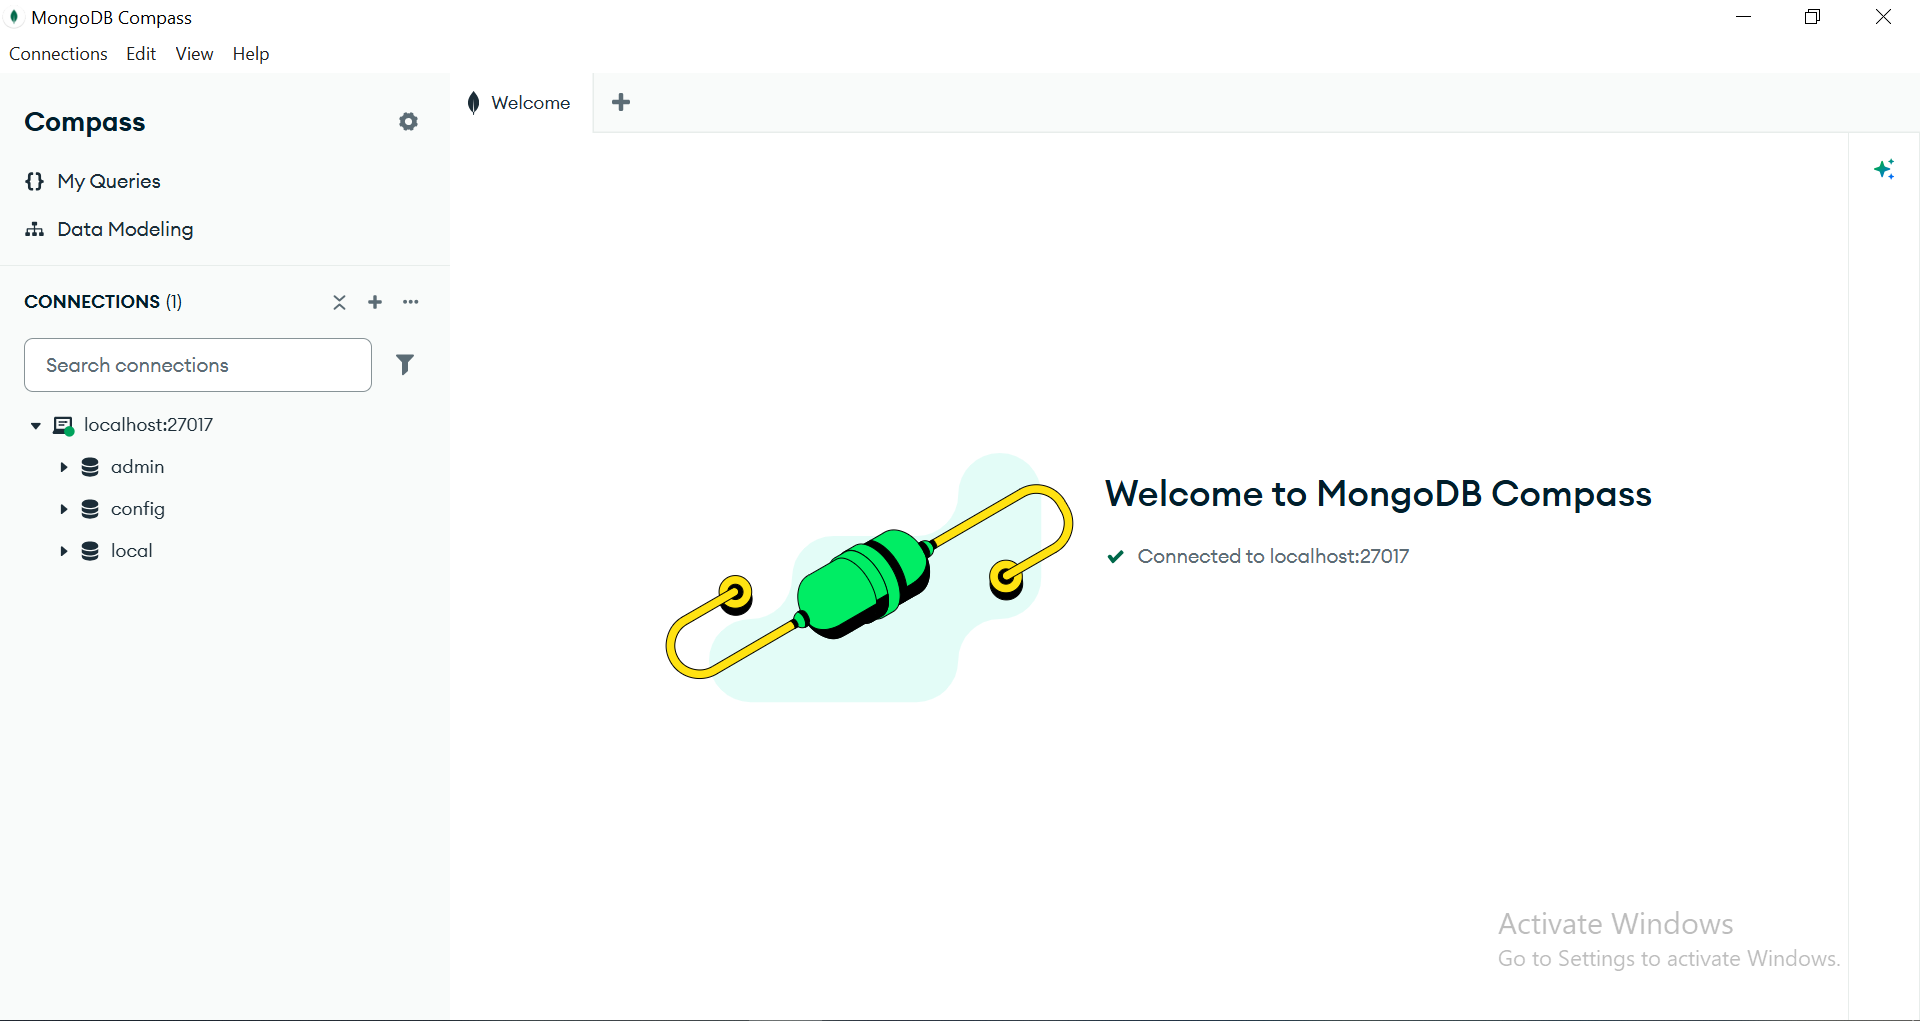
\includegraphics[width=\linewidth]{nicelyConnected.png}
    \caption*{Connection Successful}
  \end{subfigure}

\end{figure}


\vspace{0.75cm}


\subsection{Create DataBase \& Its Collections}

\begin{prettyBox}{Create}{myblue}
    \begin{itemize}
        \item We first create a new data base "Query\_TP"
        \item Then we add 2 collections "Sportif" \& "Gym"
    \end{itemize}
\end{prettyBox}

\vspace{0.25cm}
\begin{figure}[H]
  \begin{subfigure}[H]{.4\textwidth}
    \centering
    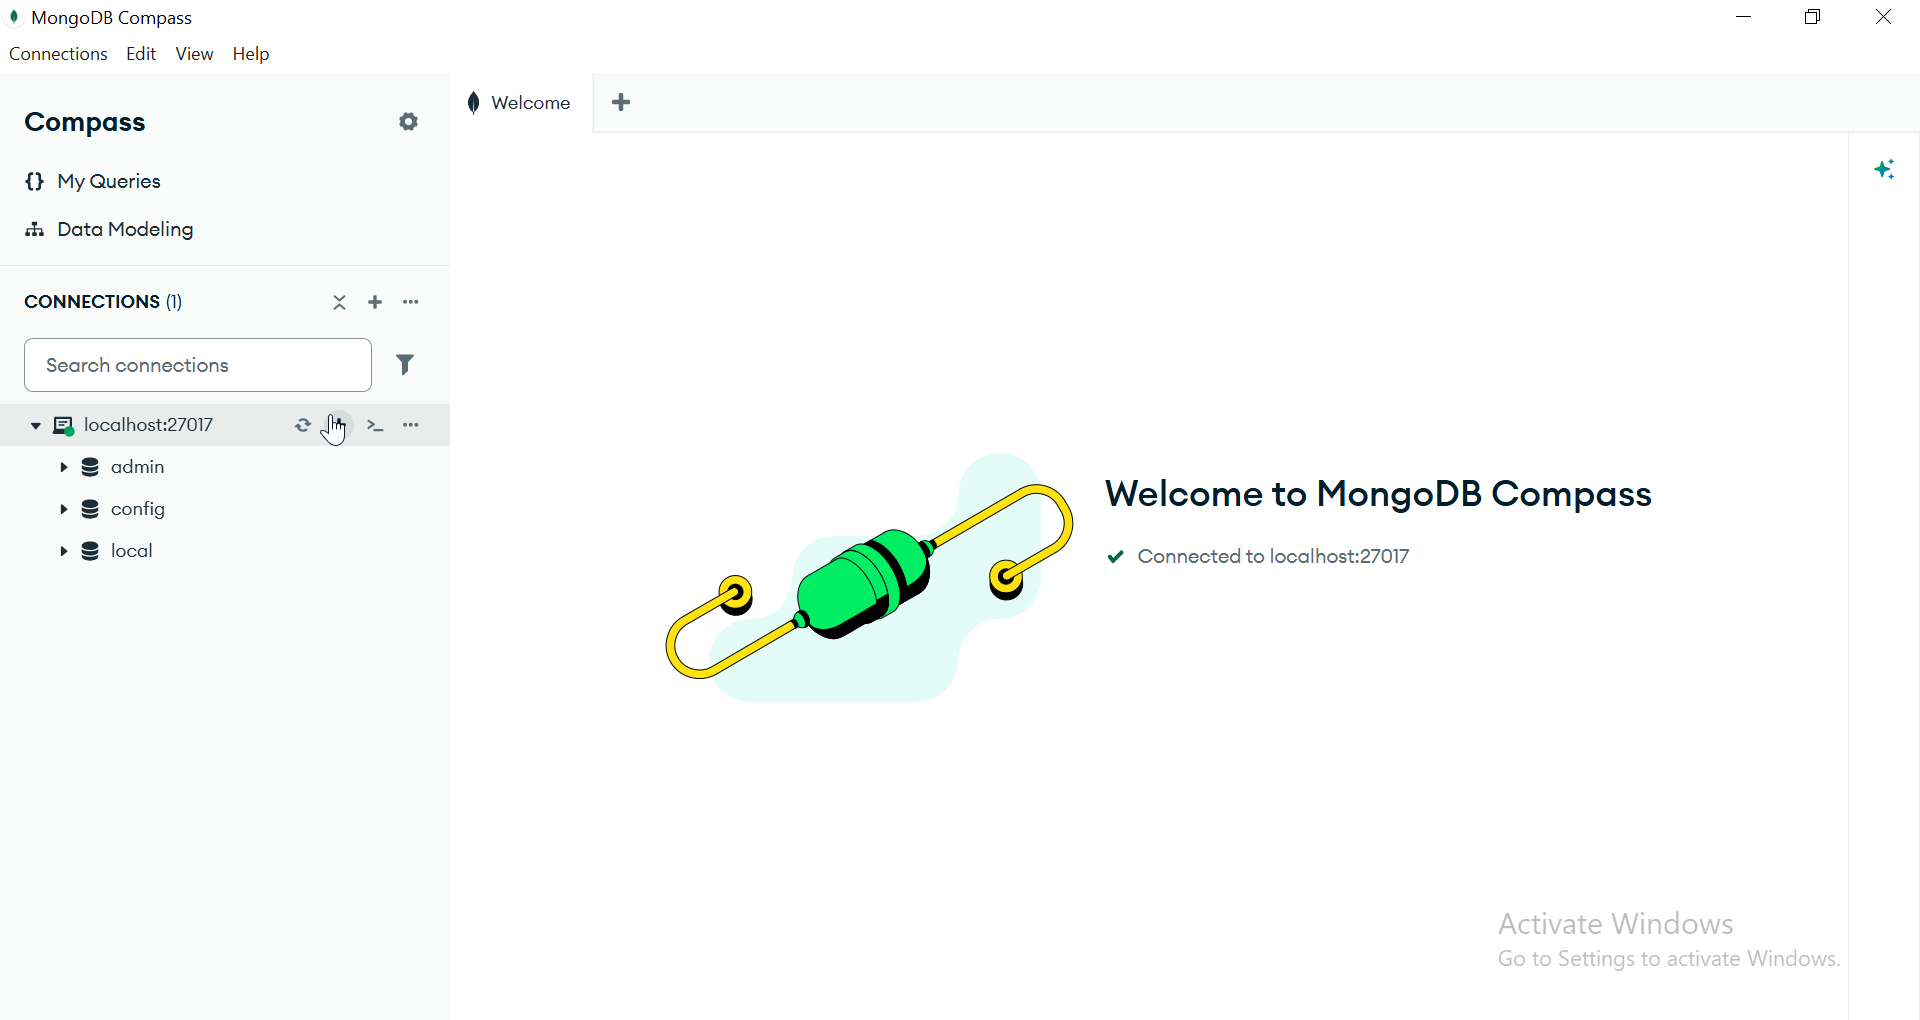
\includegraphics[width=\linewidth]{create1.png}
    \caption*{Click Create New Data Base}
  \end{subfigure}
  \hfill
  \begin{subfigure}[H]{.4\textwidth}
    \centering
    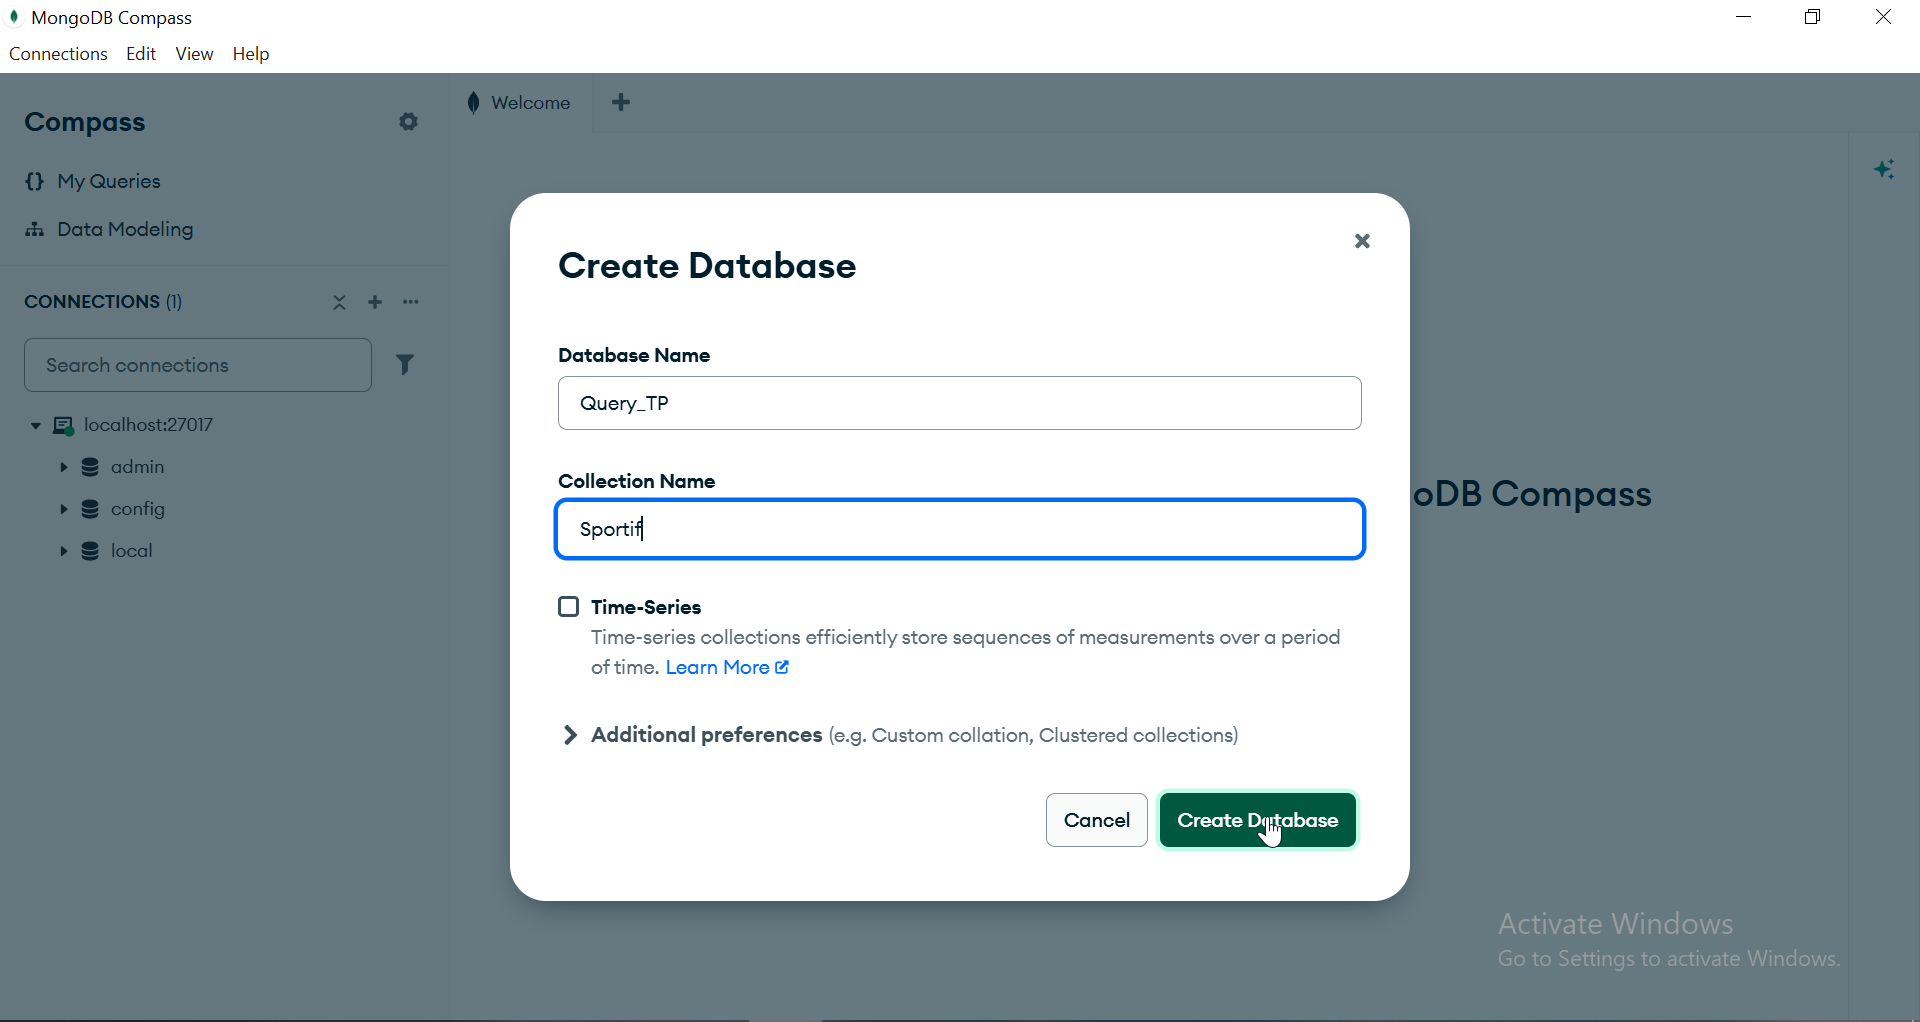
\includegraphics[width=\linewidth]{create2.png}
    \caption*{Input Data Base Name \& Collection}
  \end{subfigure}

  \medskip

  \begin{subfigure}[H]{.4\textwidth}
    \centering
    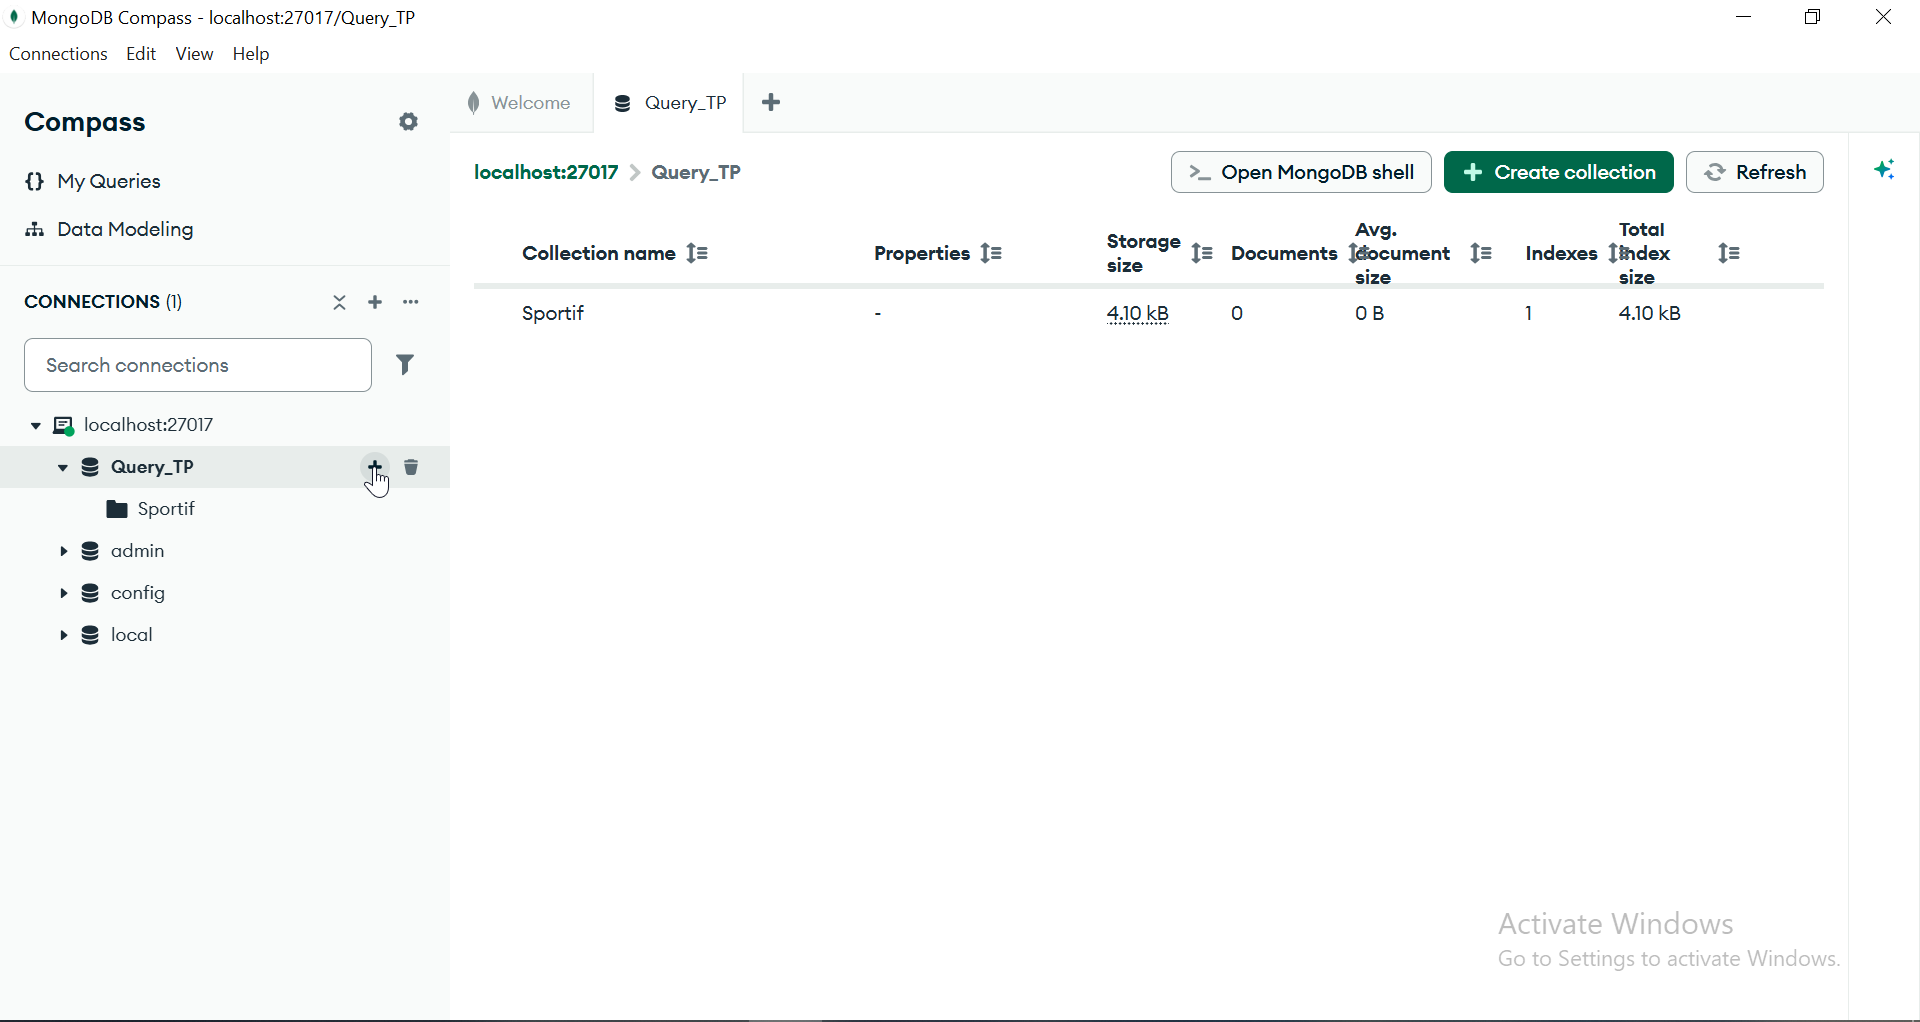
\includegraphics[width=\linewidth]{create3.png}
    \caption*{Click Create New Collection}
  \end{subfigure}
  \hfill
  \begin{subfigure}[H]{.4\textwidth}
    \centering
    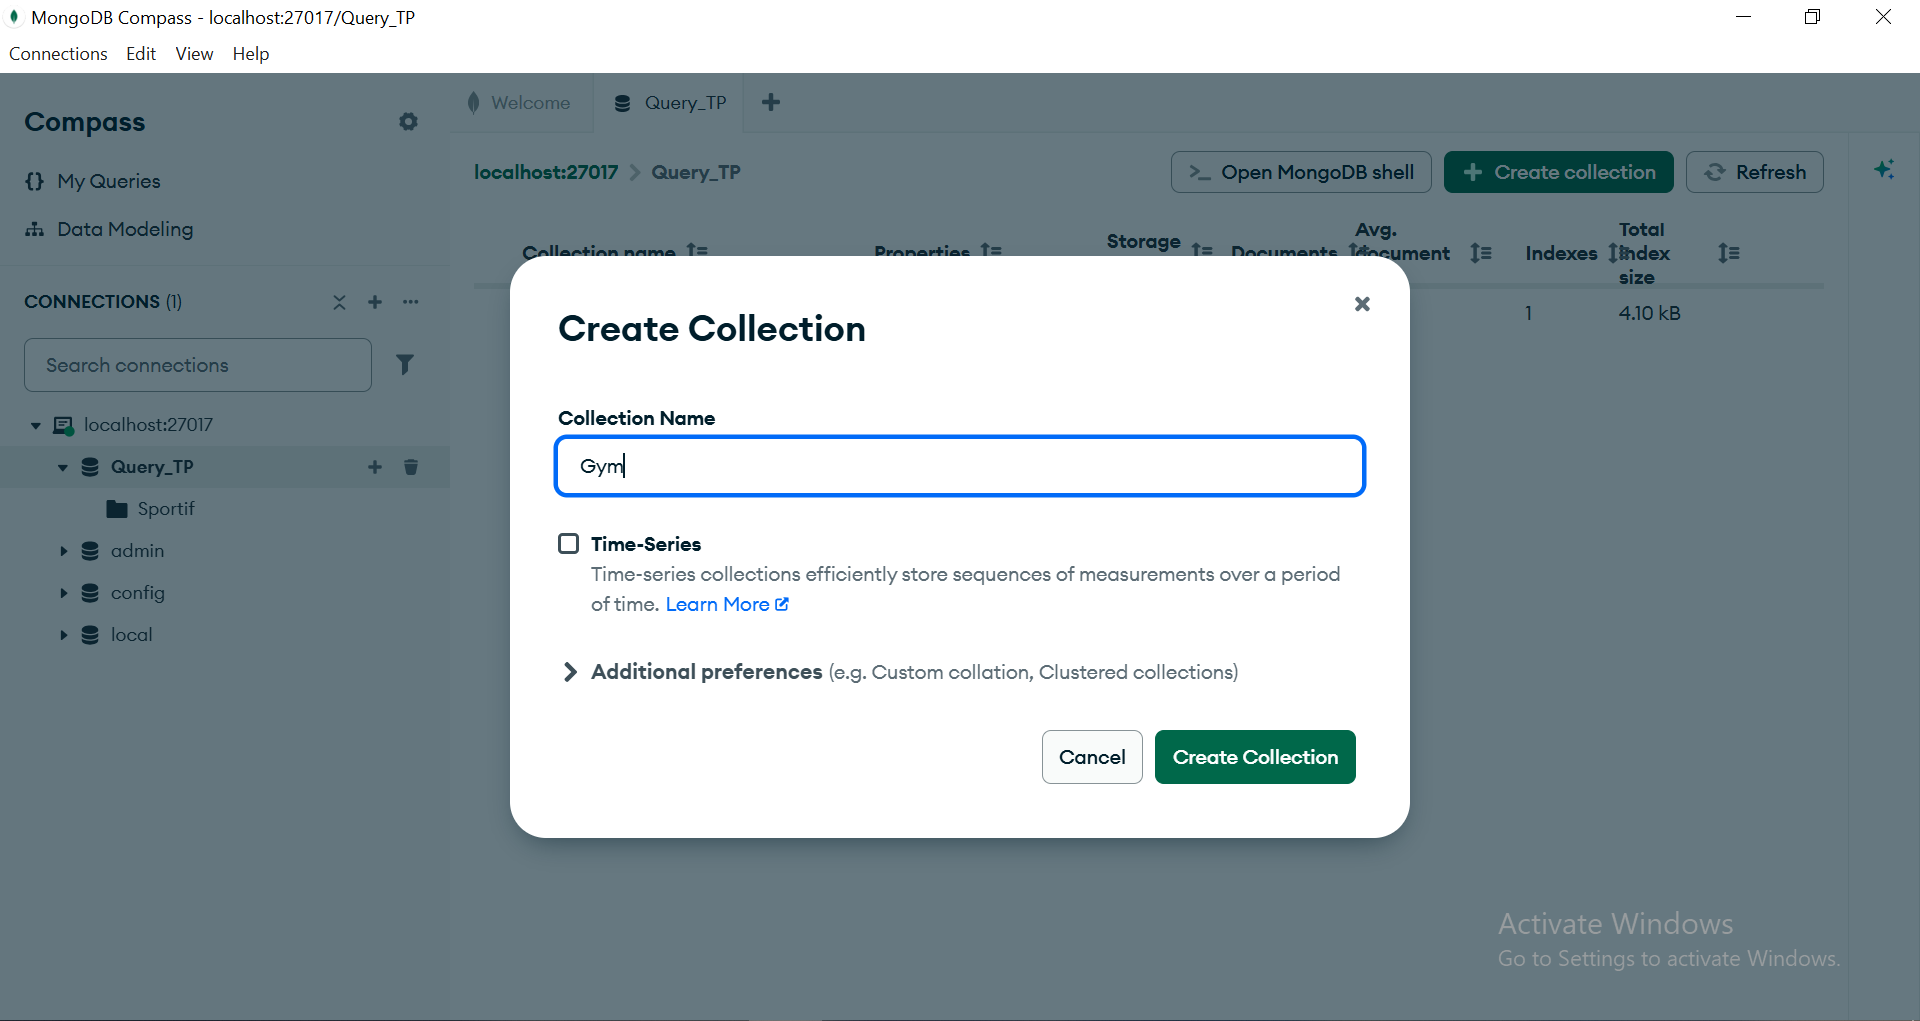
\includegraphics[width=\linewidth]{create4.png}
    \caption*{Input Name Of Second Collection}
  \end{subfigure}
\end{figure}




\subsection{Import Json Document}
\begin{prettyBox}{Import}{myblue}
    \begin{itemize}
        \item Download the json files from the link \href{https://drive.google.com/drive/u/0/folders/1QhHWxjCT5Tyiqe-nFsuYfgtquzwoyzJ4}{https://drive.google.com/drive/u/0/folders/1QhHWxjCT5Tyiqe-nFsuYfgtquzwoyzJ4} 
        \item For each collection click the import data button then select the appropriate json file
    \end{itemize}
\end{prettyBox}

\vspace{0.25cm}

\begin{figure}[H]
  \begin{subfigure}[H]{.4\textwidth}
    \centering
    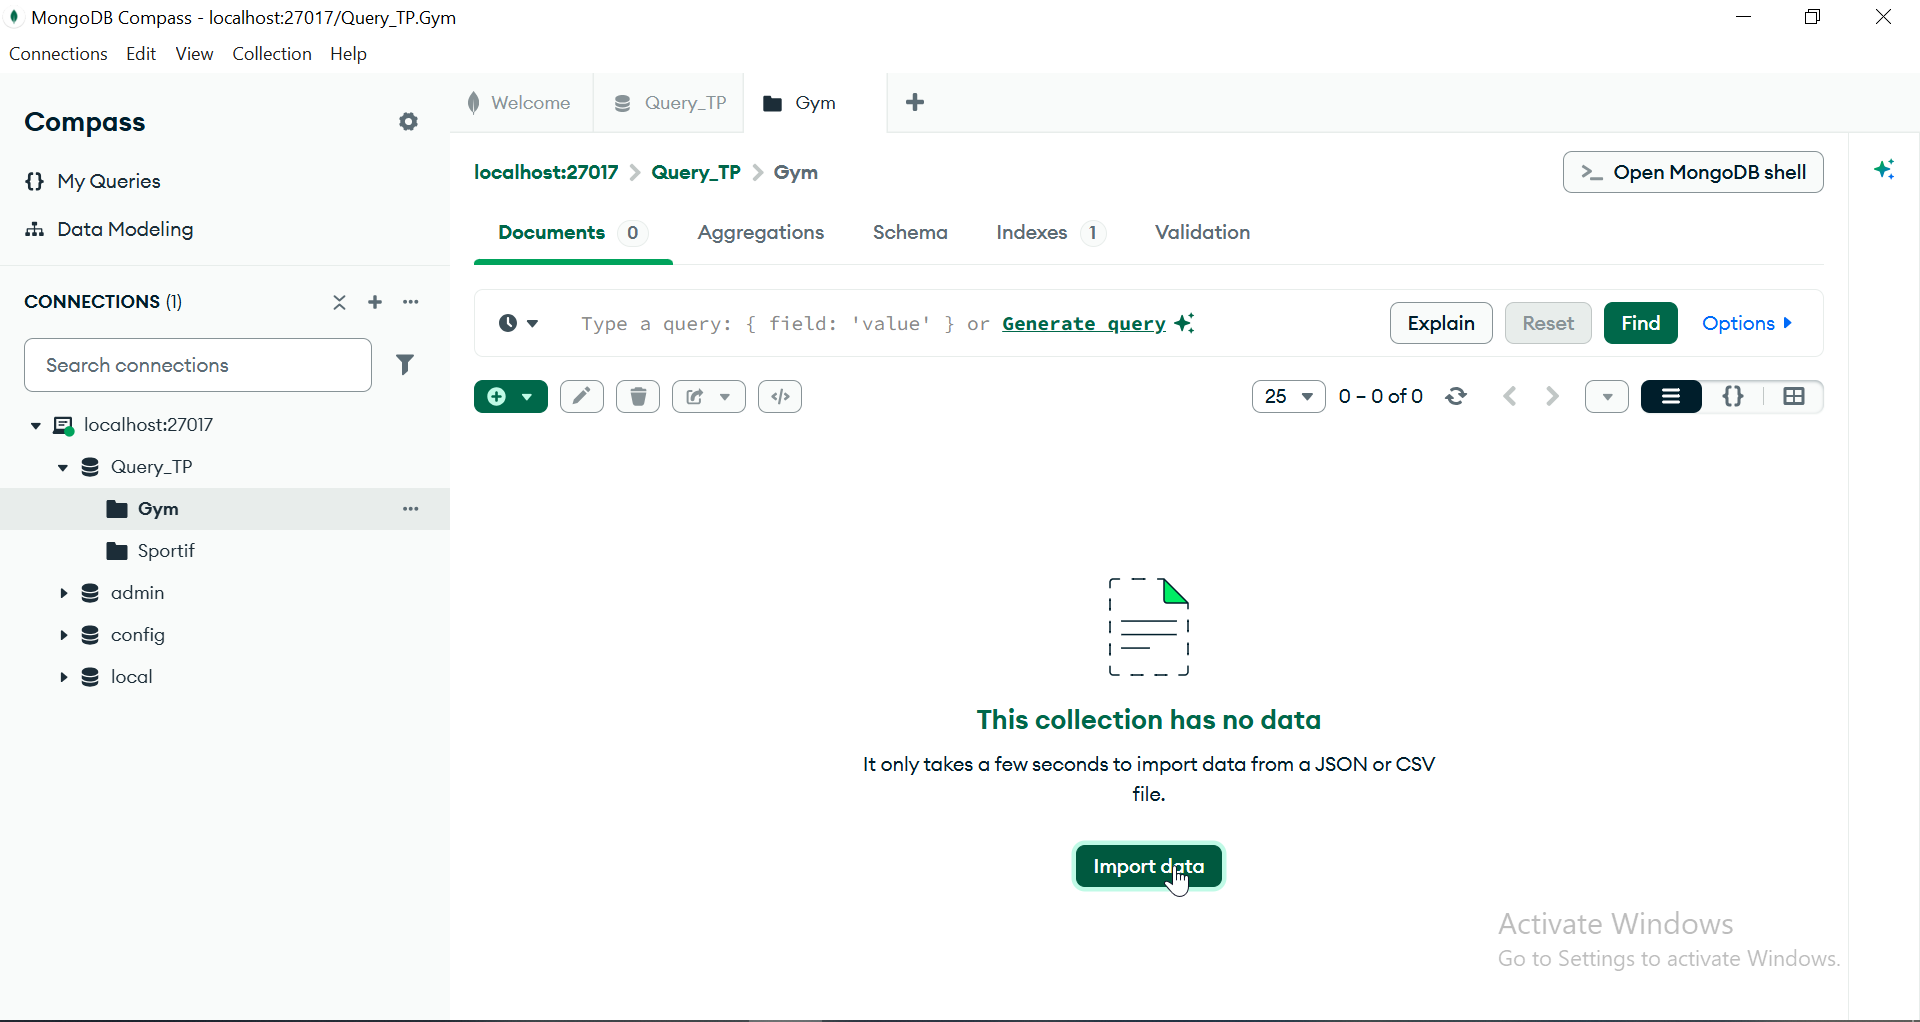
\includegraphics[width=\linewidth]{import1.png}
    \caption*{Click On Import Data}
  \end{subfigure}
  \hfill
  \begin{subfigure}[H]{.4\textwidth}
    \centering
    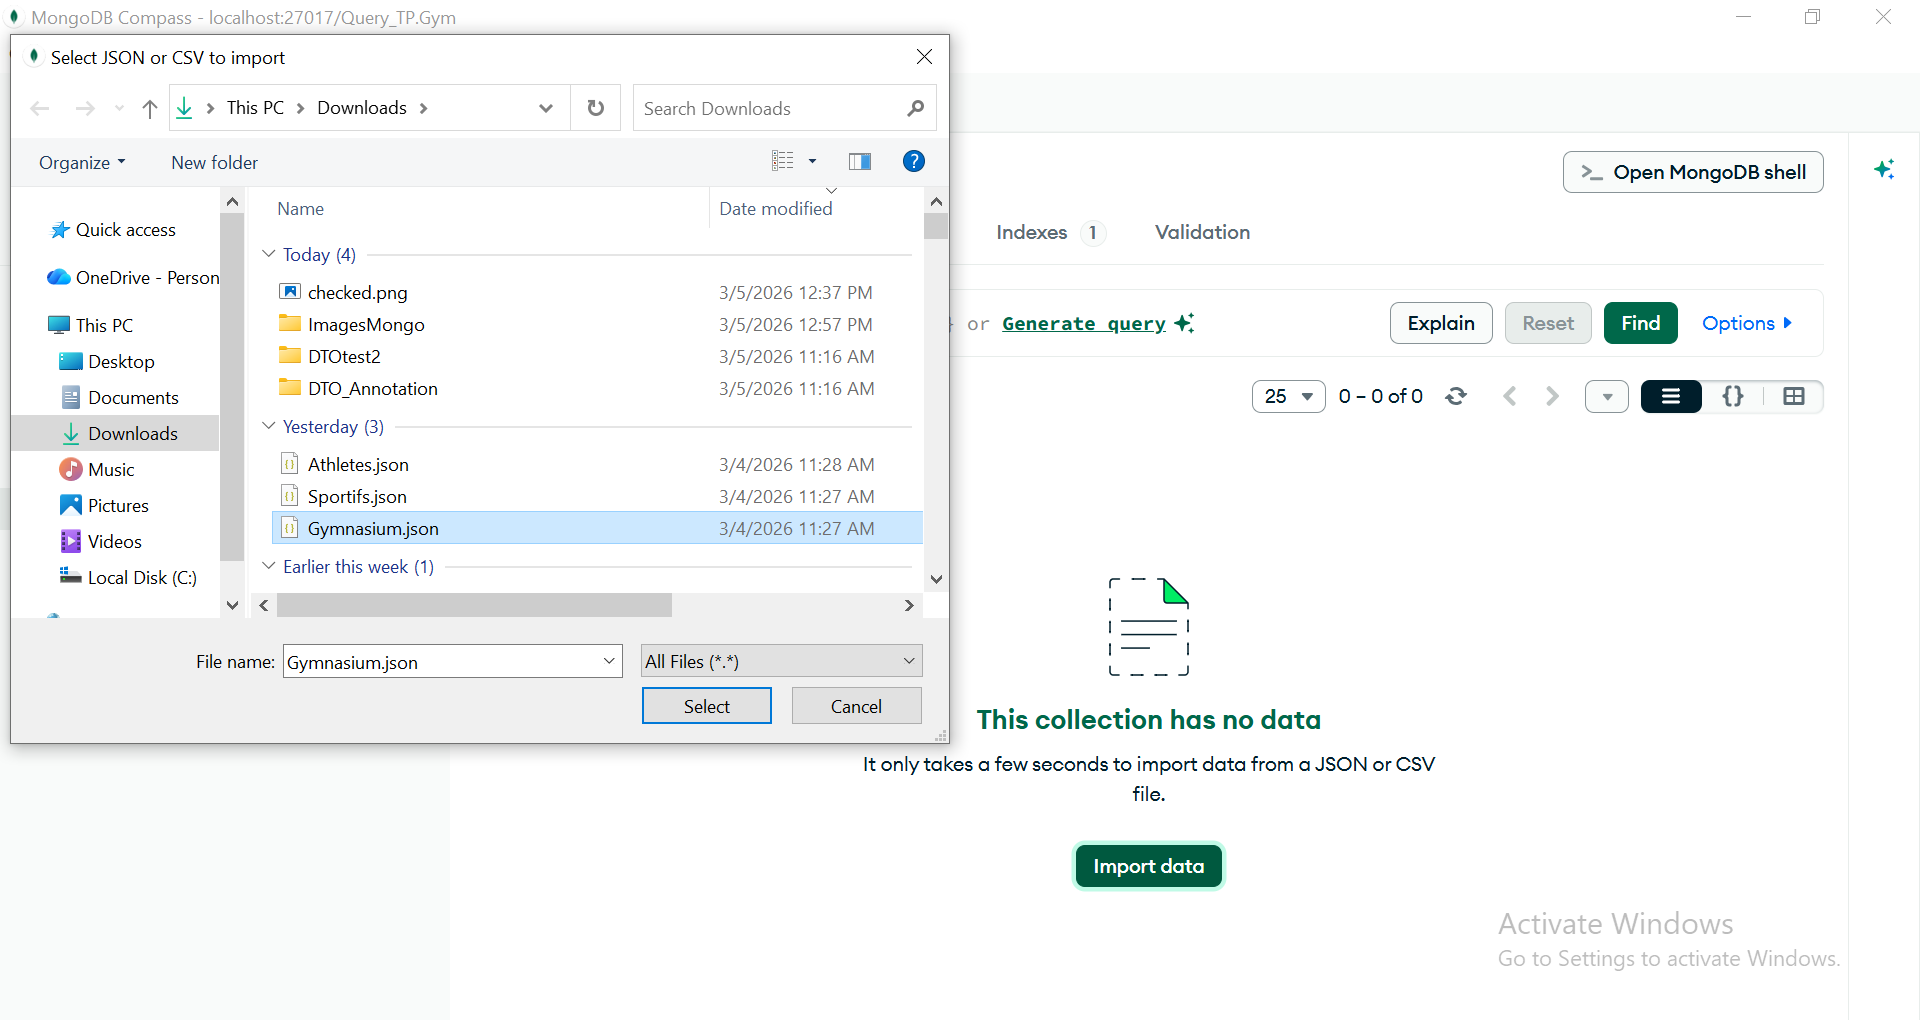
\includegraphics[width=\linewidth]{import2.png}
    \caption*{Select Json Document}
  \end{subfigure}

  \medskip
 
  \center
  \begin{subfigure}[H]{.4\textwidth}
    \centering
    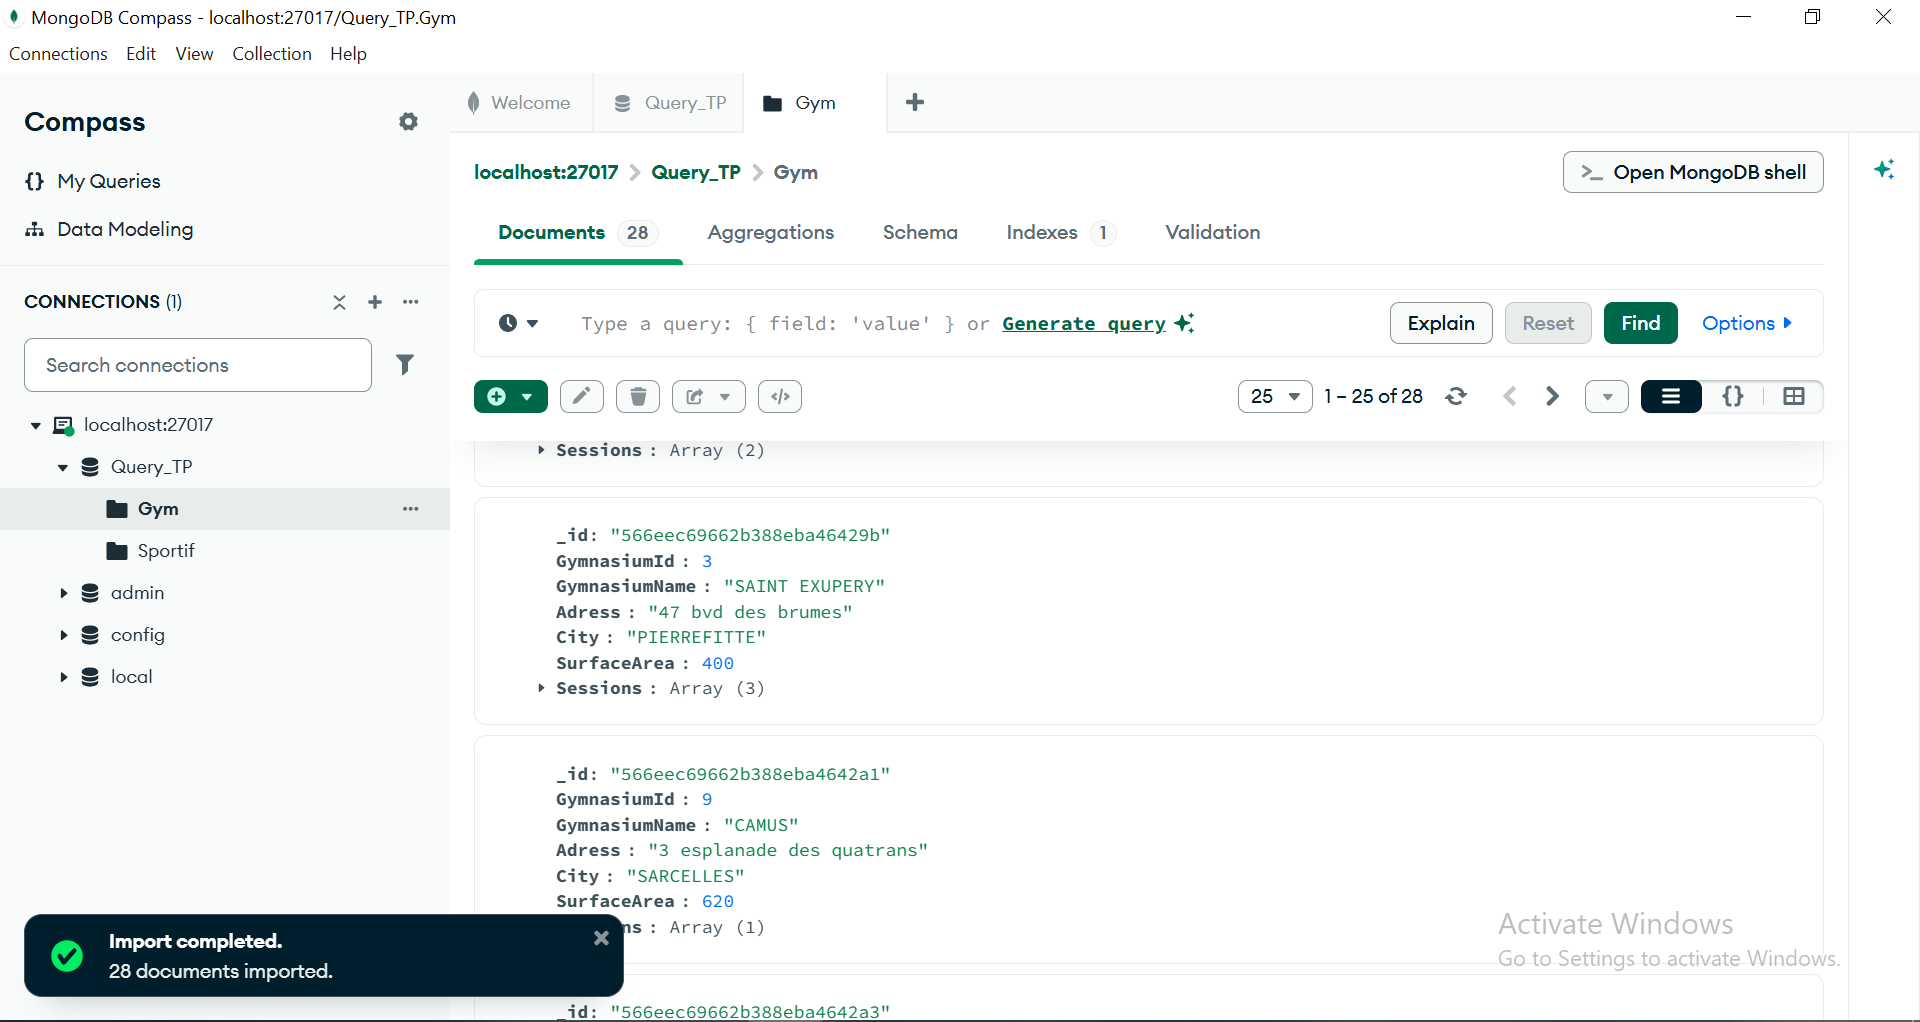
\includegraphics[width=\linewidth]{import3.png}
    \caption*{Import Completed}
  \end{subfigure}
\end{figure}



\vspace{0.5cm}


\subsection{Open The Shell}
\begin{prettyBox}{Shell}{myblue}
    \begin{itemize}
        \item Click on the button open mongoDB shell
        \item Make sure to switch to the data base we created
    \end{itemize}
\end{prettyBox}

\vspace{0.25cm}
\begin{figure}[H]
  \begin{subfigure}[H]{.4\textwidth}
    \centering
    
\includegraphics[width=\linewidth]{sh.png}
    \caption*{Click On Open MongoDB Shell}
  \end{subfigure}
  \hfill
  \begin{subfigure}[H]{.4\textwidth}
    \centering
    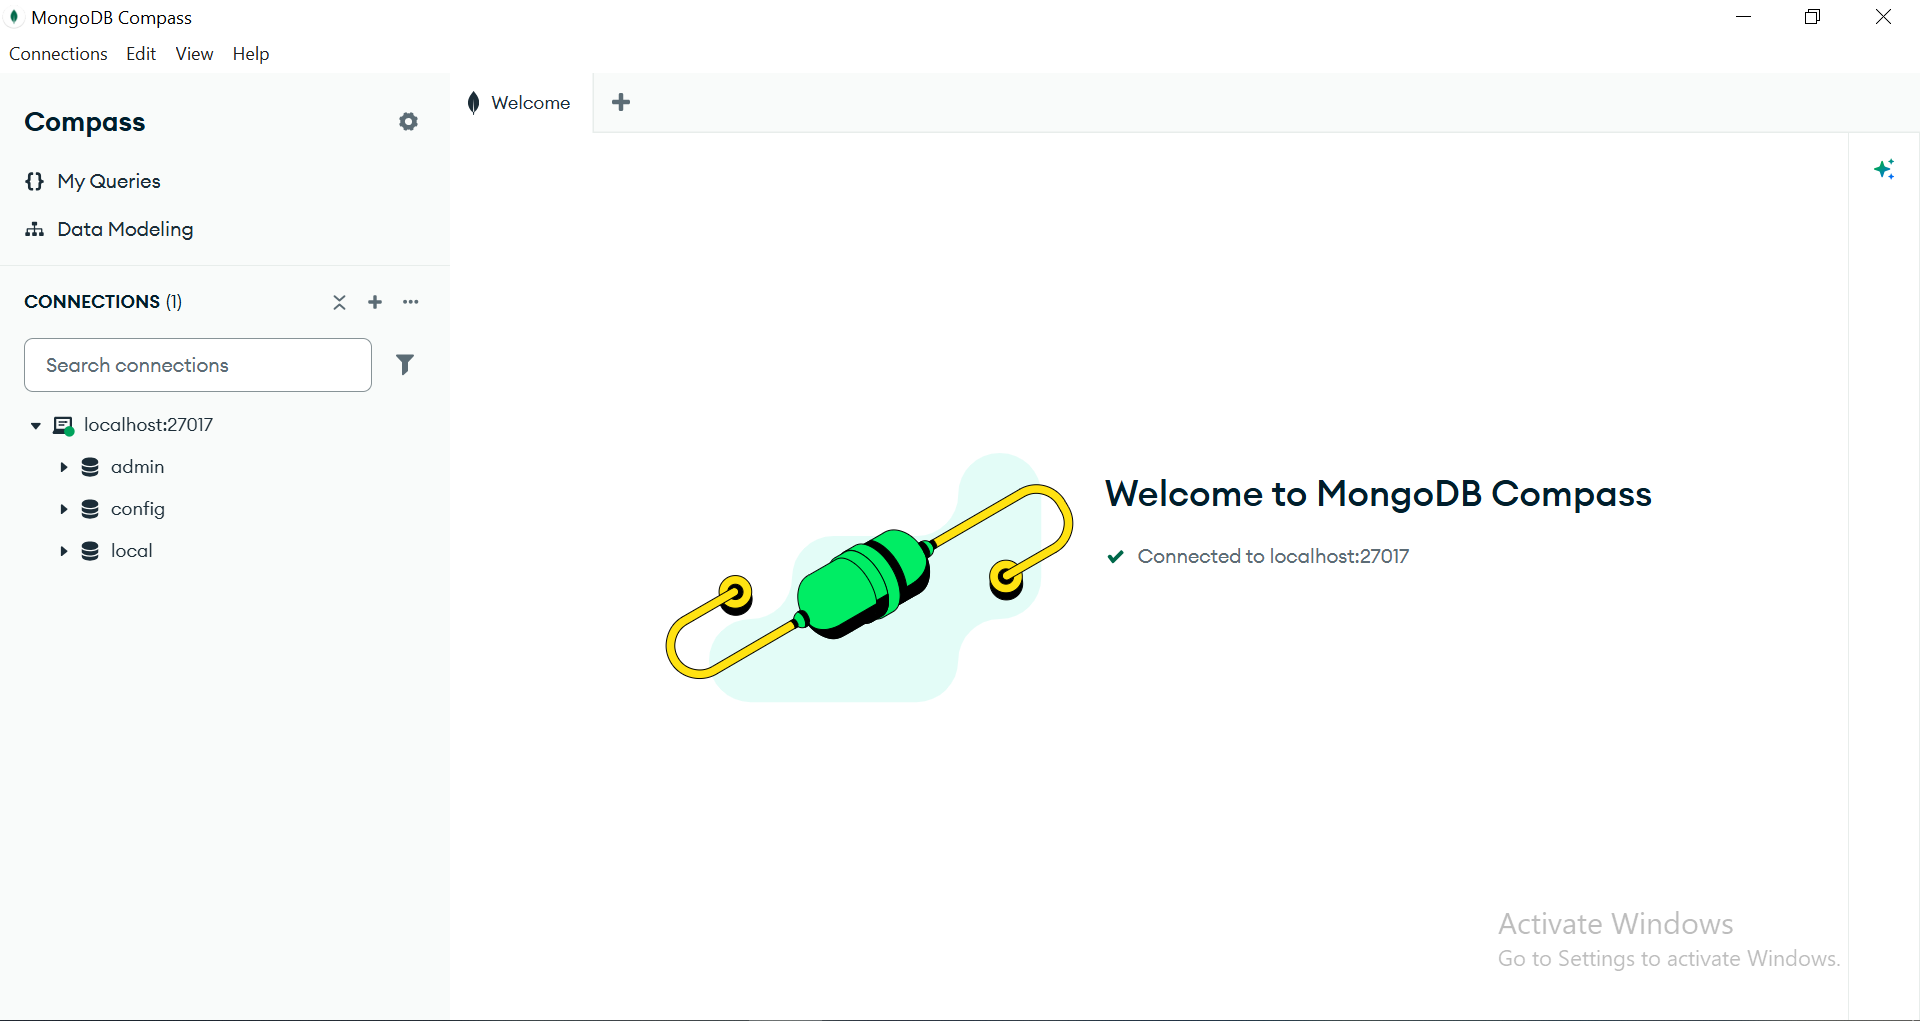
\includegraphics[width=\linewidth]{nicelyConnected.png}
    \caption*{Switch To The Data Base We Created}
  \end{subfigure}

\end{figure}




\section{Queries}

\subsection{Sportifs That Are Between The Age Of 20 - 30}

\begin{codeInput}{javascript}{Age 20-30}{code01}
// first method implicit and 
db["Sportif"].find({"Age" : {$gte : 20 , $lte : 30}} , {"Nom" : 1 , "Age" : 1, "_id": 0})

// second method explicit and
db["Sportif"].find( { 
    $and : [
        {"Age" : {$gte : 20} } , 
        {"Age" : {$lte : 30} } 
    ]
    } , 
    {"Nom" : 1 , "Age" : 1, "_id": 0}
)
\end{codeInput}

\vspace{0.25cm}

\subsection{Gyms From The Villetaneuse Or Sarcelles City \& Surface Greater Than 400}

\begin{codeInput}{javascript}{Gym In Villetaneuse Or Sarcelles , And Surface \(>\) 400}{code01}
// first method using in operator
db["Gym"].find({ 
    "City" : { 
        $in : [/SARCELLES/i, /VILLETANEUSE/i] 
    }, 
    "SurfaceArea" : {$gt : 400}
})

// second method using or operator
db["Gym"].find({
    $or : [ 
        {"City" :/SARCELLES/i}, 
        {"City" :/VILLETANEUSE/i}
    ] , 
    "SurfaceArea" : {$gt : 400}
})
\end{codeInput}

\vspace{0.25cm}
\subsection{Sportifs That Practise Volley Ball}

\begin{codeInput}{javascript}{Gyms Volley Ball}{code01}
db["Sportif"].find( {"Sports.Jouer" : /Volley ball/i}, {"_id" : 0 , "Nom" : 1} )
\end{codeInput}

\subsection{Name Of Gyms \& Day That Volley Ball Sessions}

\begin{codeInput}{javascript}{Gyms Volley Ball}{code01}
db["Gym"].find({"Sessions.Label" : /Volley ball/i } , {"Sessions.Day" : 1 , "GymnasiumName" : 1})
\end{codeInput}

\vspace{0.25cm}
\subsection{Same As Previous Query But Session Is On Wednesday After 15h}

\begin{codeInput}{javascript}{Gyms Volley Ball Session On Wednesday After 15h}{code01}
// first method implicit and 
db["Gym"].find({
    "Sessions.Label" : /Volley ball/i  , 
    "Sessions.Day" : /Mercredi/i , 
    "Sessions.Time" : {$gt : 15 } 
    },
    {"_id" : 0, "GymnasiumName" : 1, "Sessions.Time" : 1}
)
\end{codeInput}

\newpage


\begin{codeInput}{javascript}{Gyms Volley Ball Session On Wednesday After 15h}{code01}
// second method explicit and 
db["Gym"].find({
    $and : [
    {"Sessions.Label" : /Volley ball/i}  , 
    {"Sessions.Day" : /Mercredi/i} , 
    {"Sessions.Time" : {$gt : 15 }} 
    ]
    },
    {"_id" : 0, "GymnasiumName" : 1, "Sessions.Time" : 1}
)
\end{codeInput}



\vspace{0.25cm}
\subsection{Sportifs That Practise Nothing}

\begin{codeInput}{javascript}{Practise Nothing}{code01}
db["Sportif"].find({
    $or : [
        {"Sports.Jouer" : {$exists : false} }, 
        {"Sports.Jouer" : {$size : 0} }
    ] 
    },
    {"_id" : 0, "Nom" : 1 , "Prenom" : 1}
)
\end{codeInput}




\end{document}

